\documentclass{article}

\usepackage{fullpage}
\usepackage{url}
\usepackage{bbm}
\usepackage{graphicx}
\usepackage{amsmath}
\usepackage{physics}
\usepackage{mathtools}
\usepackage{bbold}
\usepackage{slashed}
\usepackage{pxfonts}
\usepackage{multicol}
\usepackage{mathptmx}
\usepackage{simplewick}
\usepackage{placeins}
\usepackage{booktabs}
\usepackage{tikz}
\usepackage[compat=1.1.0]{tikz-feynman}

\usepackage{lmodern}
\usepackage[T1]{fontenc}
\usepackage[fontsize=13.5pt]{fontsize}

\DeclareMathOperator{\erfi}{erfi}
\newcommand{\R}{\ensuremath{\mathbb{R}}}
\newcommand{\C}{\ensuremath{\mathbb{C}}}

\tikzset{
  counterterm/.style={
    circle,
    draw,
    inner sep=1pt,
    minimum size=3mm,
    path picture={
      \draw[black] 
      (path picture bounding box.south west) -- (path picture bounding box.north east)
      (path picture bounding box.south east) -- (path picture bounding box.north west);
    }
  }
}

\title{QFT1 Formulas}

\begin{document}
\maketitle

\section{A scalar with a higher-derivative kinetic term}
\subsection{The scaling dimension of the coupling constant}
Since the action is a scalar, and must have $[S] = 0$, then the Lagrangian must have $[\mathcal{L}] = d$. The kinetic term then has:
\begin{equation}
    \left[
        \frac{1}{2}((\partial_\mu\partial^\mu + m^2)\phi)((\partial_\nu\partial^\nu + m^2)\phi)
    \right] = 2\cdot2 + 2[\phi] = d
\end{equation}
\begin{equation}
    \left[\phi\right] = \frac{d}{2} - 2
\end{equation}
The interaction term, then, has a dimension:
\begin{equation}
    \left[\frac{\lambda}{4!}\phi^4\right] = [\lambda] + 4[\phi] = d
\end{equation}
\begin{equation}
    [\lambda] + 4\left(\frac{d}{2} - 2\right) = d
\end{equation}
\begin{equation}
    [\lambda] = 8 - d
\end{equation}
Sanity check:
\begin{center}
\begin{tabular}{ c c c }
    $d = 4$ & $[\phi] = 0$ & $[\lambda] = 4$ \\ \hline
    $d = 6$ & $[\phi] = 1$ & $[\lambda] = 2$ \\ \hline
    $d = 8$ & $[\phi] = 2$ & $[\lambda] = 0$
\end{tabular}
\end{center}
\subsection{Additional terms for the $m = 0$ case}
For $m = 0$, the theory reduces to
\begin{equation}
    \mathcal{L} = \frac{1}{2}\left(\partial^\mu\partial_\mu\phi\right)\left(\partial^\nu\partial_\nu\phi\right) - \frac{\lambda}{4!}\phi^4
\end{equation}
It still retains the $\mathbb{Z}_2$ symmetry $\phi \rightarrow -\phi$, and thus only operators with even powers of $\phi$ are allowed. For the case where the coupling constant is dimensionless $d = 8$, the by construction the highest power of $\phi$ that can appear in any term is $\phi^4$, since $\left[\phi^4\right] = 4[\phi] = 8$. This leaves only the terms that mix $\phi$ and its derivative up to that power.
\newline
For $\phi^4$ term, there can't be any additional derivatives, since every derivative adds a scaling dimension, and $\phi^4$ already has the maximal relevant scaling dimension. For $\phi^2$, there are two additional terms: the one with no derivatives, with total scaling dimension $[\phi^2] = 4$, and the one with a single deLamberian (we can only use derivatives in deLamberians $\partial^\mu\partial_\mu$ to preserve Lorentz invariance), which has scaling dimension $\left[\left(\partial^\mu\partial_\mu\phi\right)\phi\right] = 6$
\begin{equation}
    \mathcal{L} = \frac{1}{2}\left(\partial^\mu\partial_\mu\phi\right)\left(\partial^\nu\partial_\nu\phi\right) - \frac{\lambda}{4!}\phi^4 + g_2 \phi^2 + g_3 \left(\partial^\mu\partial_\mu\phi\right)\phi
\end{equation}
These, of course, match the two terms we removed when setting the mass to zero. In the $m \ne 0$ case, $g_2 = 2m^2$ and $g_3 = m^4$.
\subsection{The scalar propegator in this theory}
As the hint implies, we can take the kinetic term, multiply it by 2, then take its inverse in momentum space. This gives:
\begin{equation}
    S(k) = \langle \phi(k) \phi(-k) \rangle = \frac{i}{k^4 + 2m^2k^2 + m^4}
\end{equation}
\subsection{The $2 \rightarrow 2$ scattering amplitude at order $\lambda$}
The interaction acts similarly to the regular real scalar $\phi^4$ interaction, and therefore it has the regular interaction vertex, with the same resultant value:
\begin{center}
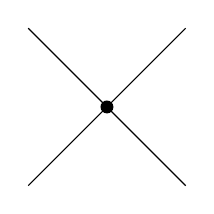
\begin{tikzpicture}[baseline=(current bounding box.center)]
  \begin{feynman}
    \vertex[dot] (v) at (0,0) {};
    \vertex (i1) at (-1, -1);
    \vertex (i2) at (-1, 1);
    \vertex (f1) at (1, 1);
    \vertex (f2) at (1, -1);
    \draw[plain] (i1) -- (v);
    \draw[plain] (i2) -- (v);
    \draw[plain] (v) -- (f1);
    \draw[plain] (v) -- (f2);
  \end{feynman}
\end{tikzpicture}
\begin{equation}
    = -i\lambda (2\pi)^8 \delta^{(8)}\left(\sum p_i\right)
\end{equation}
\end{center}
And so:
\begin{equation}
    \mathcal{M} = -\lambda
\end{equation}
\subsection{The $2 \rightarrow 2$ scattering amplitude at order $\lambda^2$}
At the next order, we simply add the three channels $s, t, u$:
\begin{center}
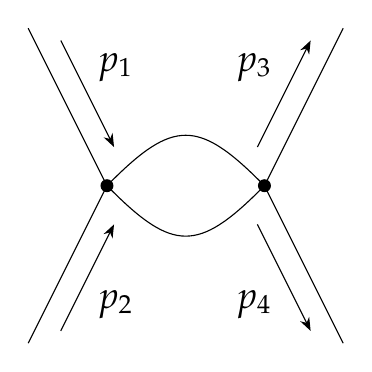
\begin{tikzpicture}[baseline=(current bounding box.center)]
  \begin{feynman}
    \vertex[dot] (v1) at (-1,0) {};
    \vertex[dot] (v2) at (1,0) {};
    \vertex (i1) at (-2, -2);
    \vertex (i2) at (-2, 2);
    \vertex (f1) at (2, 2);
    \vertex (f2) at (2, -2);
    \draw[plain, momentum=$p_1$] (i2) -- (v1);
    \draw[plain, momentum'=$p_2$] (i1) -- (v1);
    \draw[plain, momentum=$p_3$] (v2) -- (f1);
    \draw[plain, momentum'=$p_4$] (v2) -- (f2);
    \draw[plain] (v1) to[out=45, in=135, looseness=1.5] (v2);
    \draw[plain] (v1) to[out=-45, in=-135, looseness=1.5] (v2);
  \end{feynman}
\end{tikzpicture}
\hspace{1cm}
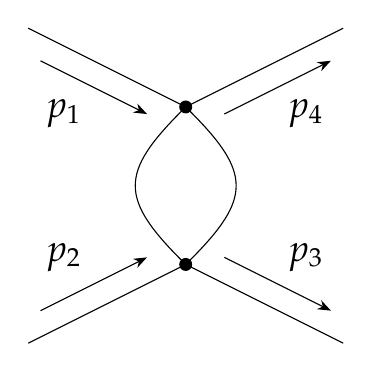
\begin{tikzpicture}[baseline=(current bounding box.center)]
  \begin{feynman}
    \vertex[dot] (v1) at (0,-1) {};
    \vertex[dot] (v2) at (0,1) {};
    \vertex (i1) at (-2, -2);
    \vertex (i2) at (-2, 2);
    \vertex (f1) at (2, -2);
    \vertex (f2) at (2, 2);
    \draw[plain, momentum'=$p_1$] (i2) -- (v2);
    \draw[plain, momentum=$p_2$] (i1) -- (v1);
    \draw[plain, momentum=$p_3$] (v1) -- (f1);
    \draw[plain, momentum'=$p_4$] (v2) -- (f2);
    \draw[plain] (v1) to[out=45, in=-45, looseness=1.5] (v2);
    \draw[plain] (v1) to[out=135, in=-135, looseness=1.5] (v2);
  \end{feynman}
\end{tikzpicture}
\hspace{1cm}
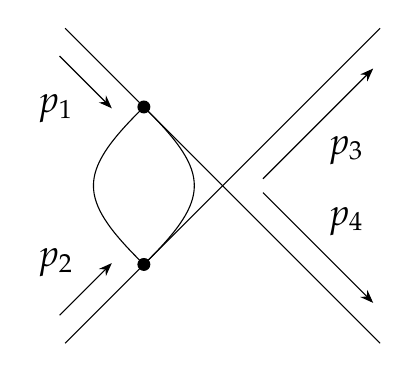
\begin{tikzpicture}[baseline=(current bounding box.center)]
  \begin{feynman}
    \vertex (i1) at (-2, -2);
    \vertex (i2) at (-2, 2);
    \vertex (f1) at (2, 2);
    \vertex (f2) at (2, -2);
    \vertex[dot] (v1) at (-1, 1) {};
    \vertex[dot] (v2) at (-1, -1) {};
    \vertex (v0) at (0,0);
    \draw[plain, momentum'=$p_1$] (i2) -- (v1);
    \draw[plain, momentum=$p_2$] (i1) -- (v2);
    \draw[plain, momentum'=$p_3$] (v0) -- (f1);
    \draw[plain, momentum=$p_4$] (v0) -- (f2);
    \draw[plain] (v2) -- (v0);
    \draw[plain] (v1) -- (v0);
    \draw[plain] (v2) to[out=45, in=-45, looseness=1.5] (v1);
    \draw[plain] (v2) to[out=135, in=-135, looseness=1.5] (v1);
  \end{feynman}
\end{tikzpicture}
\end{center}
The second order contribution from these three diagrams is:
\begin{equation}
\begin{gathered}
    \mathcal{M}_2 = -\lambda^2[V(s) + v(t) + V(u)]
\end{gathered}
\end{equation}
Where:
\begin{equation}
    V(p^2) = \frac{1}{2}\int \frac{d^8q}{(2\pi)^8} \frac{i^2}{(q^4 + 2m^2q^2 + m^4)((q - p)^4 + 2m^2(q - p)^2 + m^4)}
\end{equation}
\subsection{Calculating}
Dimensional Regularization! Woo :)
\newline
\subsubsection*{Identifying the divergences}
The degree of the integral is $\frac{d^8q}{q^8} \sim 1$ which means the integral is logarithmically divergent.
\subsubsection*{Changing the dimension of the momentum integral $d_0 \rightarrow d$}
\begin{equation}
    V_d(p^2) = -\frac{1}{2}\int \frac{d^dq}{(2\pi)^d} \frac{1}{(q^4 + 2m^2q^2 + m^4)((q + p)^4 + 2m^2(q - p)^2 + m^4)}
\end{equation}
\subsubsection*{Feynman's trick}
Using the given formula with
\begin{equation}
\begin{gathered}
    A = (q - p)^2 + m^2
    \qquad
    B = q^2 + m^2
    \\
    n_1 = n_2 = 2
\end{gathered}
\end{equation}
Gives:
\begin{equation}
\begin{gathered}
    \frac{1}{(q^4 + 2m^2q^2 + m^4)((q + p)^4 + 2m^2(q - p)^2 + m^4)} = \\ =
    \frac{\Gamma(4)}{\Gamma(2)^2} \int_0^1 dx \frac{x^1(1 - x)^1}{\left[x((q + p)^2 + m^2) + (1 - x)(q^2 + m^2)\right]^4} = \\ =
    \frac{3}{2} \int_0^1 dx \frac{x(1 - x)}{\left[q^2 + xp^2 + 2xqp + m^2\right]^4}
\end{gathered}
\end{equation}
This gives:
\begin{equation}
    V_d(p^2) = -\frac{3}{4}\int \frac{d^dq}{(2\pi)^d}\int_0^1 dx \frac{x(1 - x)}{\left[q^2 + xp^2 + 2xqp + m^2\right]^4}
\end{equation}
\subsubsection*{Change of variables}
Defining $l = q +xp$ and changing the order of integration:
\begin{equation}
    V_d(p^2) = -\frac{3}{4}\int_0^1 dx \int \frac{d^dl}{(2\pi)^d} \frac{x(1 - x)}{\left[l^2 + p^2(1 - x)x + m^2\right]^4}
\end{equation}
Naming the remaining part of the denominator and performing Wick's rotation $l^0 \rightarrow il_E^0$:
\begin{equation}
    \Delta = p^2(1 - x)x + m^2
\end{equation}
Gives us the well known integral:
\begin{equation}
    V_d(p^2) = -i\frac{3}{4}\int_0^1 x(1 - x)dx \int \frac{d^dl_E}{(2\pi)^d} \frac{1}{\left[l_E^2 + \Delta\right]^4}
\end{equation}
\subsubsection*{Solving the $l_E$ integral}
Using:
\begin{equation}
    \frac{d^dl_E}{(2\pi)^d} \frac{1}{(l_E^2 + \Delta)^n} = \frac{1}{(4\pi)^\frac{d}{2}}\frac{\Gamma\left(n - \frac{d}{2}\right)}{\Gamma(n)}\Delta^{\frac{d}{2} - n}
\end{equation}
We get:
\begin{equation}
    V_d(p^2) = -i\frac{\Gamma\left(4 - \frac{d}{2}\right)}{8(4\pi)^\frac{d}{2}}\int_0^1 x(1 - x)dx\Delta^{\frac{d}{2} - 4}
\end{equation}
\subsubsection*{Using dimension $d = 8 - \epsilon$}
Set the dimension $d = 8 - \epsilon$:
\begin{equation}
    V(p^2) = -i\frac{\Gamma\left(\frac{\epsilon}{2}\right)}{8(4\pi)^4}\int_0^1 x(1 - x)dx\left(\frac{\Delta}{4\pi}\right)^{-\frac{\epsilon}{2}}
\end{equation}
Using the approximation of $\Gamma$ and of powers of $\Delta$:
\begin{equation}
    \Gamma\left(\frac{\epsilon}{2}\right) = \frac{2}{\epsilon} - \gamma + \mathcal{O}(\epsilon)
\end{equation}
\begin{equation}
    \Delta^{-\frac{\epsilon}{2}} = 1 - \frac{\epsilon}{2} \ln\Delta + \mathcal{O}(\epsilon^2)
\end{equation}
This gives:
\begin{equation}
    V(p^2) = -\frac{i}{8(4\pi)^4}\int_0^1 x(1 - x)dx\left(\frac{2}{\epsilon} - \gamma - \ln\left(\frac{\Delta}{4\pi}\right) + \mathcal{O}(\epsilon)\right)
\end{equation}
Pluggin $\Delta$ back in:
\begin{equation}
    V(p^2) = -\frac{i}{8(4\pi)^4}\int_0^1 x(1 - x)dx\left(\frac{2}{\epsilon} - \gamma - \ln\left(\frac{p^2(1 - x)x + m^2}{4\pi}\right) + \mathcal{O}(\epsilon)\right)
\end{equation}
\subsection{Renormalization and the beta function}
Defining the physical constant:
\begin{equation}
    \lambda_p = \mathcal{M}(s = t = u = M^2)
\end{equation}
For some energy scale $M$, we can renormalize the above by simply writing the physical coupling as a funciton of bare coupling:
\begin{equation}
    \lambda_p = \lambda - \lambda^2\cdot 3V(M^2) + \mathcal{O}(\lambda^3)
\end{equation}
Flip the expansion:
\begin{equation}
    \lambda = \lambda_p + \lambda_p^2\cdot 3V(M^2)
\end{equation}
And plug it into the general $2\rightarrow2$ scattering amplitude:
\begin{equation}
\begin{gathered}
    \mathcal{M}_{2\rightarrow2} = \lambda - \lambda^2\left[V(s) + V(t) + V(u)\right] + \mathcal{O}(\lambda^3) = \\ = \lambda_p - \lambda_p^2\left[V(s) + V(t) + V(u) - 3V(M^2)\right] + \mathcal{O}(\lambda^3) = \\ = \lambda_p - \frac{\lambda_p^2}{8(4\pi)^4}\int_0^1 x(1 - x)dx\Bigg(\ln\frac{x(1-x)s + m^2}{M^2(1 - x)x + m^2} + \\ + \ln\frac{x(1-x)t + m^2}{M^2(1 - x)x + m^2} + \ln\frac{x(1-x)u + m^2}{M^2(1 - x)x + m^2}\Bigg) + \mathcal{O}(\lambda^3, \epsilon)
\end{gathered}
\end{equation}
Now, to get the beta function, we just need to take the coupling from the flipped expansion, and derive it by $M$:
\begin{equation}
\begin{gathered}
    \beta(\lambda) = M \frac{d\lambda}{dM} = M\lambda^2\frac{dV(M^2)}{dM} = M\frac{\lambda^2}{8(4\pi)^4} \int_0^1x(1 - x) dx \frac{2M}{x(1 - x)M^2 + m^2} = \\ =
    \frac{\lambda^2}{1024\pi^4} \int_0^1 \frac{x(1 - x)}{x(1 - x) + \frac{m^2}{M^2}} dx
\end{gathered}
\end{equation}
For high energy $M^2 \gg m^2$, this becomes:
\begin{equation}
    \beta(\lambda) = \frac{\lambda^2}{1024\pi^4}
\end{equation}
Which is positive, so the coupling constant becomes larger as the energy scale grows, meaning that theory is valid for low energies and is not asymptotically free.
\subsection{The RG flow of the massless theory}
As we lower the energy cutoff $\Lambda$ (or raise the energy scale $M$), some operators will become irrelevant and some will remain. For the massless theory, we chose from the beginwith to only take the relevant operators, those which dimension is smaller then $d$, so that when the theory scales down, they will grow. So, we reuqire three fine tunings, and the action will look like the one we saw in section 2.
\end{document}